\documentclass[10pt]{beamer}
\usepackage[english]{babel}
\usepackage[utf8]{inputenc}
\usepackage[T1]{fontenc}
\usepackage{helvet}
\usepackage{ragged2e}
%-------------------------------------------------------
% INFORMATION IN THE TITLE PAGE
%-------------------------------------------------------

\newcommand{\cstitle}{\textbf{Bioinformatics}}
\subtitle[]{Phylogenetic trees}
\newcommand{\cscourseCode}{1005155}
\newcommand{\csauthor}{MSc. Vicente Machaca Arceda}
\institute[UNSA]{Universidad Nacional de San Agustín de Arequipa}
\newcommand{\csemail}{vmachacaa@unsa.edu.pe}
\newcommand{\instituteabr}{UNSA}
\newcommand{\nameUp}{ICC Fase 1}
\date{\today}
\title[\cscourseCode]{\cstitle}
\author{\csauthor}
%%%%%%%%%%%%%%%%%

%-------------------------------------------------------
% CHOOSE THE THEME
%-------------------------------------------------------
\def\mycmd{0} % CS THEME
%\def\mycmd{1} % MYTHEME
%-------------------------------------------------------


\if\mycmd1
\usetheme[]{Feather}
\newcommand{\chref}[2]{	\href{#1}{{\usebeamercolor[bg]{Feather}#2}} }
\else
\usepackage{csformat}
\fi

\newcommand{\1}{
	\setbeamertemplate{background}{
		
\includegraphics[width=\paperwidth,height=\paperheight]{img/1}
		\tikz[overlay] \fill[fill opacity=0.75,fill=white] (0,0) rectangle (-\paperwidth,\paperheight);
	}
}



%-------------------------------------------------------
% THE BODY OF THE PRESENTATION
%-------------------------------------------------------

\begin{document}
	
	
	\AtBeginSubsection[]
	{
		\begin{frame}
			\frametitle{Table of Contents}
			\tableofcontents[currentsubsection]
		\end{frame}
	}
	
	
	%-------------------------------------------------------
	% THE TITLEPAGE
	%-------------------------------------------------------
	
	\if\mycmd1 % MY THEME
	\1{
		\begin{frame}[plain,noframenumbering] 
			\titlepage 
		\end{frame}}
		\else % CS THEME
		\maketitle
		\fi

%-------------------------------------------------------
%-------------------------------------------------------
\begin{frame}{Table of Contents}
\tableofcontents
\end{frame}
%-------------------------------------------------------
%-------------------------------------------------------

%%%%%%%%%%%%%%%%%%%%%%%%%%%%%%%%%%%%%%%%%%%%%%%%%%%%%%%%%%%%%%%%%%%%%%%%%%%%%%%%%%%%%%%%%%%%%%%%%%%%%%%%%%%%%%%%
%%%%%%%%%%%%%%%%%%%%%%%%%%%%%%%%%%%%%%%%%%%%%%%%%%%%%%%%%%%%%%%%%%%%%%%%%%%%%%%%%%%%%%%%%%%%%%%%%%%%%%%%%%%%%%%%
\section{Introduction}
%%%%%%%%%%%%%%%%%%%%%%%%%%%%%%%%%%%%%%%%%%%%%%%%%%%%%%%%%%%%%%%%%%%%%%%%%%%%%%%%%%%%%%%%%%%%%%%%%%%%%%%%%%%%%%%%
%%%%%%%%%%%%%%%%%%%%%%%%%%%%%%%%%%%%%%%%%%%%%%%%%%%%%%%%%%%%%%%%%%%%%%%%%%%%%%%%%%%%%%%%%%%%%%%%%%%%%%%%%%%%%%%%

%%%%%%%%%%%%%%%%%%%%%%%%%%%%%%%%%%%%%%%%%%%%%%%%%%%%%%%%%%%%%%%%%%%%%%%%%%%%%%%%%%%%%%%%%%%%%%%%%%%%%%%%%%%%%%%%
%%%%%%%%%%%%%%%%%%%%%%%%%%%%%%%%%%%%%%%%%%%%%%%%%%%%%%%%%%%%%%%%%%%%%%%%%%%%%%%%%%%%%%%%%%%%%%%%%%%%%%%%%%%%%%%%
\subsection{Objectives}
%%%%%%%%%%%%%%%%%%%%%%%%%%%%%%%%%%%%%%%%%%%%%%%%%%%%%%%%%%%%%%%%%%%%%%%%%%%%%%%%%%%%%%%%%%%%%%%%%%%%%%%%%%%%%%%%
%%%%%%%%%%%%%%%%%%%%%%%%%%%%%%%%%%%%%%%%%%%%%%%%%%%%%%%%%%%%%%%%%%%%%%%%%%%%%%%%%%%%%%%%%%%%%%%%%%%%%%%%%%%%%%%%

%-------------------------------------------------------
%-------------------------------------------------------
\begin{frame}{Introduction}{Objectives}
\begin{itemize}
    \item<1-> Understand the importance of phylogenetic trees. 
    \item<2-> Understand and implement UPGMA.
  \end{itemize}
\end{frame}
%-------------------------------------------------------
%-------------------------------------------------------


%%%%%%%%%%%%%%%%%%%%%%%%%%%%%%%%%%%%%%%%%%%%%%%%%%%%%%%%%%%%%%%%%%%%%%%%%%%%%%%%%%%%%%%%%%%%%%%%%%%%%%%%%%%%%%%%
%%%%%%%%%%%%%%%%%%%%%%%%%%%%%%%%%%%%%%%%%%%%%%%%%%%%%%%%%%%%%%%%%%%%%%%%%%%%%%%%%%%%%%%%%%%%%%%%%%%%%%%%%%%%%%%%
\section{Phylogenetics}
%%%%%%%%%%%%%%%%%%%%%%%%%%%%%%%%%%%%%%%%%%%%%%%%%%%%%%%%%%%%%%%%%%%%%%%%%%%%%%%%%%%%%%%%%%%%%%%%%%%%%%%%%%%%%%%%
%%%%%%%%%%%%%%%%%%%%%%%%%%%%%%%%%%%%%%%%%%%%%%%%%%%%%%%%%%%%%%%%%%%%%%%%%%%%%%%%%%%%%%%%%%%%%%%%%%%%%%%%%%%%%%%%

%%%%%%%%%%%%%%%%%%%%%%%%%%%%%%%%%%%%%%%%%%%%%%%%%%%%%%%%%%%%%%%%%%%%%%%%%%%%%%%%%%%%%%%%%%%%%%%%%%%%%%%%%%%%%%%%
%%%%%%%%%%%%%%%%%%%%%%%%%%%%%%%%%%%%%%%%%%%%%%%%%%%%%%%%%%%%%%%%%%%%%%%%%%%%%%%%%%%%%%%%%%%%%%%%%%%%%%%%%%%%%%%%
\subsection{Definition}
%%%%%%%%%%%%%%%%%%%%%%%%%%%%%%%%%%%%%%%%%%%%%%%%%%%%%%%%%%%%%%%%%%%%%%%%%%%%%%%%%%%%%%%%%%%%%%%%%%%%%%%%%%%%%%%%
%%%%%%%%%%%%%%%%%%%%%%%%%%%%%%%%%%%%%%%%%%%%%%%%%%%%%%%%%%%%%%%%%%%%%%%%%%%%%%%%%%%%%%%%%%%%%%%%%%%%%%%%%%%%%%%%

%-------------------------------------------------------
%-------------------------------------------------------
\begin{frame}{Phylogenetics}{Definition}
	\begin{block}{}
		Phylogenetics is the study of the evolutionary history of living organisms using tree like diagrams to represent pedigrees of these organisms \cite{xiong2006essential}. 		
	\end{block}
\end{frame}
%-------------------------------------------------------
%-------------------------------------------------------

%-------------------------------------------------------
%-------------------------------------------------------
\begin{frame}{Phylogenetics}{Example}
	\begin{figure}
		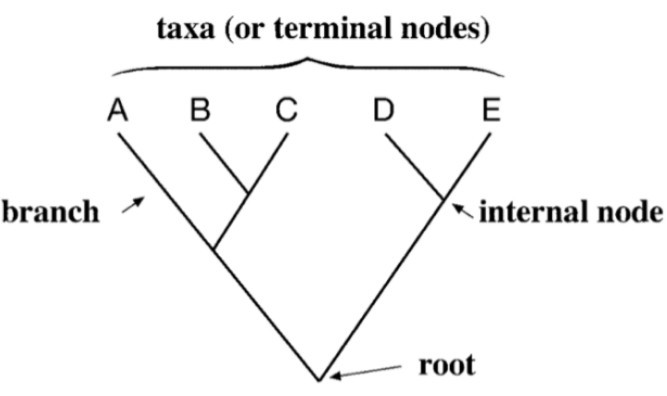
\includegraphics[width=0.7\textwidth]{img/philo/example_1}
		\caption{A typical bifurcating phylogenetic tree showing root, internal nodes, terminal nodes and branches. Source: \cite{xiong2006essential}}			
	\end{figure}
\end{frame}
%-------------------------------------------------------
%-------------------------------------------------------

%-------------------------------------------------------
%-------------------------------------------------------
\begin{frame}{Phylogenetics}{Example}
	\begin{figure}
		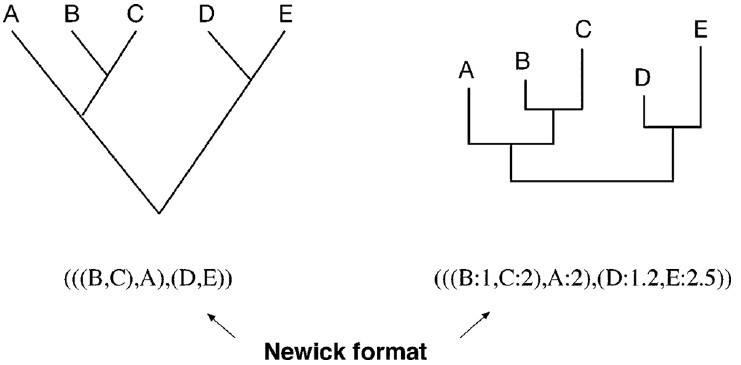
\includegraphics[width=\textwidth]{img/philo/example_2}
		\caption{Newick format of tree representation. Source: \cite{xiong2006essential}}			
	\end{figure}
\end{frame}
%-------------------------------------------------------
%-------------------------------------------------------

%-------------------------------------------------------
%-------------------------------------------------------
\begin{frame}{Phylogenetics}{Methods}
	\begin{figure}
		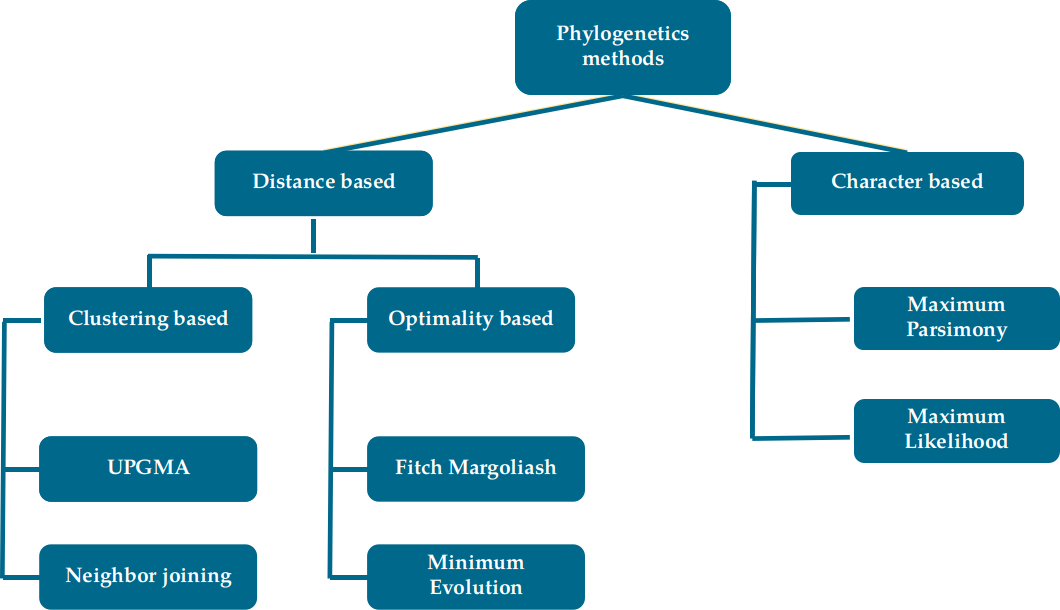
\includegraphics[width=\textwidth]{img/philo/methods}
		\caption{The most used methods to build philogenetic trees.}			
	\end{figure}
\end{frame}
%-------------------------------------------------------
%-------------------------------------------------------

%%%%%%%%%%%%%%%%%%%%%%%%%%%%%%%%%%%%%%%%%%%%%%%%%%%%%%%%%%%%%%%%%%%%%%%%%%%%%%%%%%%%%%%%%%%%%%%%%%%%%%%%%%%%%%%%
%%%%%%%%%%%%%%%%%%%%%%%%%%%%%%%%%%%%%%%%%%%%%%%%%%%%%%%%%%%%%%%%%%%%%%%%%%%%%%%%%%%%%%%%%%%%%%%%%%%%%%%%%%%%%%%%
\subsection{UPGMA}
%%%%%%%%%%%%%%%%%%%%%%%%%%%%%%%%%%%%%%%%%%%%%%%%%%%%%%%%%%%%%%%%%%%%%%%%%%%%%%%%%%%%%%%%%%%%%%%%%%%%%%%%%%%%%%%%
%%%%%%%%%%%%%%%%%%%%%%%%%%%%%%%%%%%%%%%%%%%%%%%%%%%%%%%%%%%%%%%%%%%%%%%%%%%%%%%%%%%%%%%%%%%%%%%%%%%%%%%%%%%%%%%%

%-------------------------------------------------------
%-------------------------------------------------------
\begin{frame}{UPGMA}{Unweighted Pair Group Method Using Arithmetic Average}
	\begin{columns}
		\begin{column}{0.48\textwidth}
			\begin{figure}
				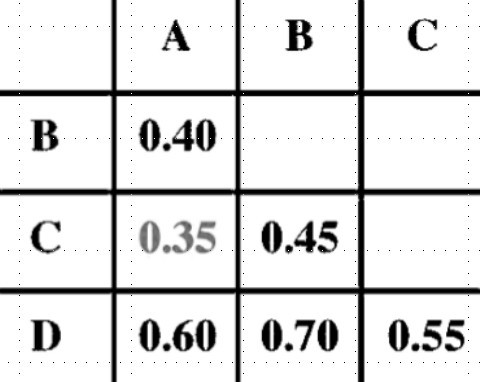
\includegraphics[width=0.8\textwidth]{img/philo/upgma_1}
				\caption{Distances between sequences (score).}
			\end{figure}
		\end{column}
		\begin{column}{0.48\textwidth}
			
			Choose the smallest distance \textit{(A, C)}. Then computer the cluster.\\ 
			
			\begin{equation*}
				\frac{AC}{2} = \frac{0.35}{2} = 0.175
			\end{equation*}			
			
			\begin{figure}
				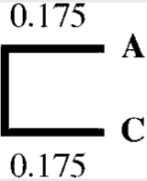
\includegraphics[width=0.3\textwidth]{img/philo/upgma_2}
			\end{figure}
			
		\end{column}
	\end{columns}

\end{frame}
%-------------------------------------------------------
%-------------------------------------------------------

%-------------------------------------------------------
%-------------------------------------------------------
\begin{frame}{UPGMA}{Unweighted Pair Group Method Using Arithmetic Average}
	Join \textit{C, A} columns. 
	\begin{columns}
		\begin{column}{0.48\textwidth}
			\begin{figure}
				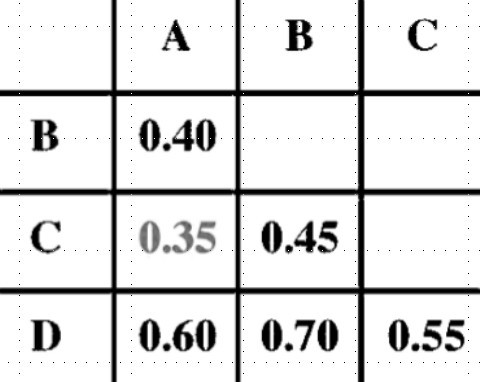
\includegraphics[width=0.8\textwidth]{img/philo/upgma_1}
				\caption{Distances between sequences (score).}
			\end{figure}
		\end{column}
		\begin{column}{0.48\textwidth}	
			\begin{figure}
				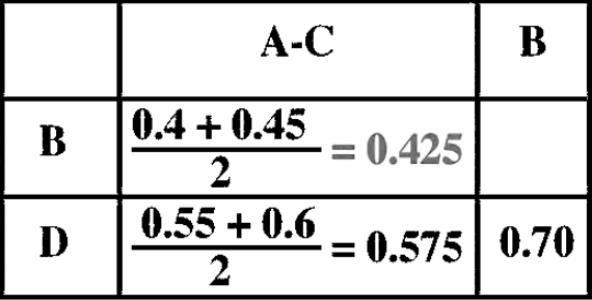
\includegraphics[width=\textwidth]{img/philo/upgma_3}
				\caption{New matrix}
			\end{figure}			
		\end{column}
	\end{columns}
	
\end{frame}
%-------------------------------------------------------
%-------------------------------------------------------

%-------------------------------------------------------
%-------------------------------------------------------
\begin{frame}{UPGMA}{Unweighted Pair Group Method Using Arithmetic Average}
	\begin{columns}
		\begin{column}{0.48\textwidth}
			\begin{figure}
				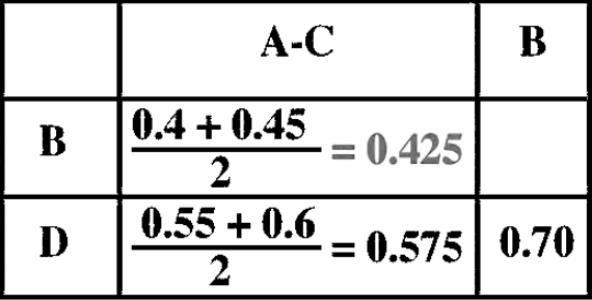
\includegraphics[width=0.8\textwidth]{img/philo/upgma_3}
				\caption{Distances between sequences (score).}
			\end{figure}
		\end{column}
		\begin{column}{0.48\textwidth}
			
			Choose the smallest distance \textit{(B, A-C)}. Then computer the cluster.\\ 					
			
			\begin{figure}
				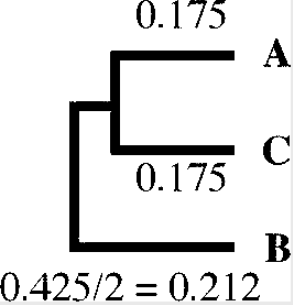
\includegraphics[width=0.6\textwidth]{img/philo/upgma_4}
			\end{figure}
			
		\end{column}
	\end{columns}
	
\end{frame}
%-------------------------------------------------------
%-------------------------------------------------------

%-------------------------------------------------------
%-------------------------------------------------------
\begin{frame}{UPGMA}{Unweighted Pair Group Method Using Arithmetic Average}
	Join \textit{AC, B} columns
	\begin{columns}
		\begin{column}{0.48\textwidth}
			\begin{figure}
				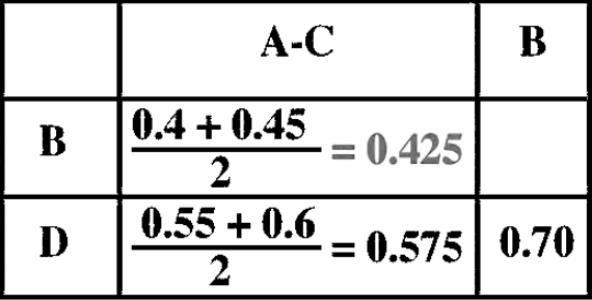
\includegraphics[width=0.8\textwidth]{img/philo/upgma_3}
				\caption{Distances between sequences (score).}
			\end{figure}
		\end{column}
		\begin{column}{0.48\textwidth}	
			\begin{figure}
				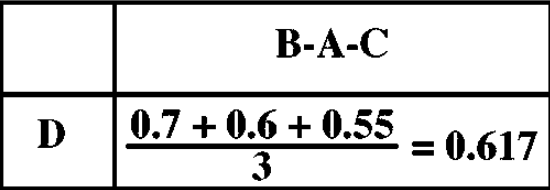
\includegraphics[width=\textwidth]{img/philo/upgma_5}
				\caption{New matrix}
			\end{figure}			
		\end{column}
	\end{columns}
	
\end{frame}
%-------------------------------------------------------
%-------------------------------------------------------



%-------------------------------------------------------
%-------------------------------------------------------
\begin{frame}{UPGMA}{Unweighted Pair Group Method Using Arithmetic Average}
	\begin{columns}
		\begin{column}{0.48\textwidth}
			\begin{figure}
				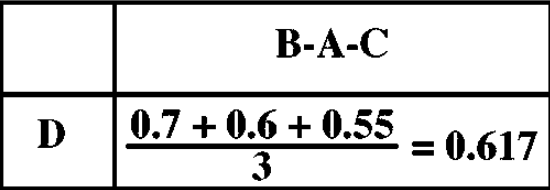
\includegraphics[width=0.8\textwidth]{img/philo/upgma_5}
				\caption{Distances between sequences (score).}
			\end{figure}
		\end{column}
		\begin{column}{0.48\textwidth}
			
			Choose the smallest distance \textit{(B-A-C)}. Then computer the cluster.\\ 					
			
			\begin{figure}
				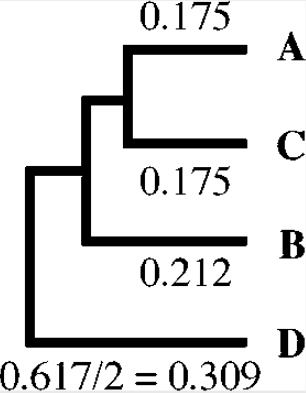
\includegraphics[width=0.6\textwidth]{img/philo/upgma_6}
			\end{figure}
			
		\end{column}
	\end{columns}
	
\end{frame}
%-------------------------------------------------------
%-------------------------------------------------------

%-------------------------------------------------------
%-------------------------------------------------------
\begin{frame}{UPGMA}{Unweighted Pair Group Method Using Arithmetic Average}
The estimated distances don’t match the actual evolutionary distances shown, which illustrates the failure of UPGMA. However, owing to its fast speed of calculation, it has found extensive usage.

	\begin{figure}
		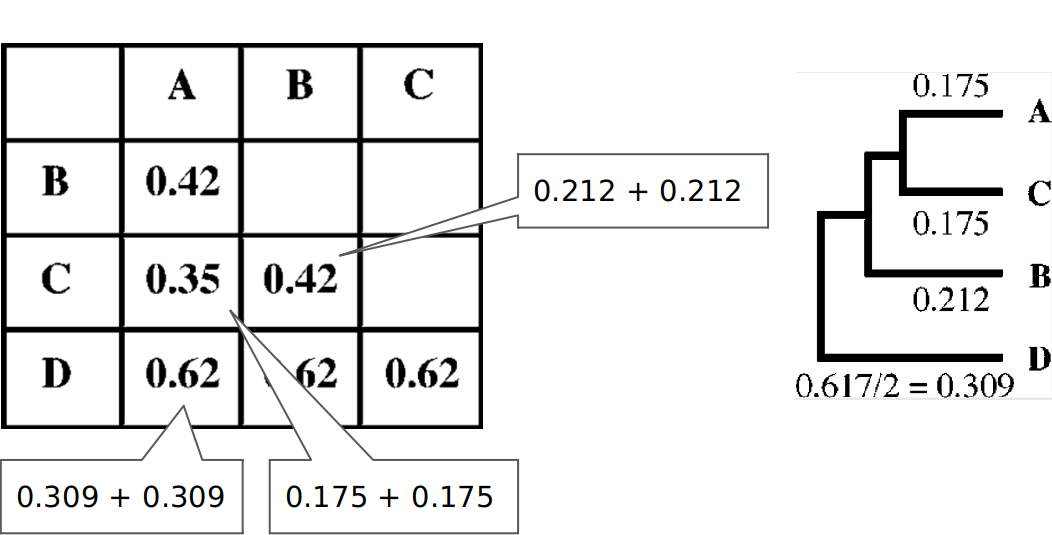
\includegraphics[width=\textwidth]{img/philo/upgma_7}
	\end{figure}
\end{frame}
%-------------------------------------------------------
%-------------------------------------------------------



%-------------------------------------------------------
%-------------------------------------------------------
\if\mycmd1 % MY THEME
\1{
	{\1
		\begin{frame}[plain,noframenumbering]
			%\finalpage{Thank you}
			\begin{figure}[]
				\centering
				
\includegraphics[width=\textwidth,height=0.7\textheight,keepaspectratio]{img/question.png}
				%\label{img:mot2}
				%\caption{Image example in 2 gray levels.}
			\end{figure}
	\end{frame}}
	\else % CS THEME
	\begin{frame}{Questions?}
		\begin{figure}[]
			\centering
			
\includegraphics[width=\textwidth,height=0.7\textheight,keepaspectratio]{img/question.png}
			%\label{img:mot2}
			%\caption{Image example in 2 gray levels.}
		\end{figure}
		
	\end{frame}
	\fi
	%-------------------------------------------------------
	%-------------------------------------------------------

%-------------------------------------------------------
%-------------------------------------------------------
\begin{frame}[allowframebreaks]
	\frametitle{References}
	%\bibliographystyle{amsalpha}
	\bibliographystyle{IEEEtran}
	\bibliography{bibliography.bib}
\end{frame}
%-------------------------------------------------------
%-------------------------------------------------------

\end{document}